% COMS 6998, Fall 2026 -- Project Proposal
% Formatting copied from main.tex; original template left intact.
% Build: latexmk -pdf neural-symbolic-proposal.tex
\documentclass[conference,10pt,letterpaper]{IEEEtran}
\usepackage[T1]{fontenc}
\usepackage{cite}
\usepackage{amsmath,amssymb}
\usepackage{graphicx}
\usepackage{tikz}
\usetikzlibrary{arrows.meta,positioning}
\usepackage{booktabs}
\usepackage{tabularx}
\usepackage{flushend}
\usepackage[hyphens]{url}
\usepackage[hidelinks]{hyperref}
\newcolumntype{Y}{>{\raggedright\arraybackslash}X}
\newcolumntype{P}[1]{>{\raggedright\arraybackslash}p{#1}}

\title{ReasonLink: Characterizing and Optimizing the\\Handoff Between Neural and Symbolic Accelerators}
\author{\IEEEauthorblockN{Vayun Gupta (vg2684), Aaron Mano Cherian (amc2535)}
\IEEEauthorblockA{COMS 6998: AI-Native Computing $\mid$ Fall 2026\\
Project Proposal $\mid$ Due October 5, 2026, 11:59 PM ET}}
\begin{document}
\maketitle
\thispagestyle{plain}
\pagestyle{plain}
\noindent\textbf{Track / topic:} A: Computing for AI; Computing Systems for Neuro-Symbolic and Compositional AI.

\section{Problem and Motivation}
Neuro-symbolic systems pair dense neural perception with irregular symbolic reasoning, and the two stages are best served by different accelerators. Between them sits a \emph{handoff}: neural outputs (e.g., class scores) must be converted into the solver's representation (variables, clauses, or assignments), moved through the memory system, and synchronized with the consumer. This handoff is usually host-CPU software and is rarely measured.

Amdahl's law applies to the glue as well as to the kernels: once both stages are accelerated, a handoff that was negligible next to slow kernels can dominate end-to-end time and leave both accelerators idle~\cite{richins2020forest,logca}. Concretely, SAT-Accel~\cite{sataccel} is loaded through a host-prepared memory image of its clause store and per-literal metadata, using a 64-byte record per literal, even when the neural stage contributes only a few bits per variable. Locating handoff time shows which interface mechanisms turn kernel speedups into system speedups.

We therefore ask: \emph{after both ends of a neuro-symbolic pipeline are accelerated, does the interface between them become the bottleneck, and if so, which interface mechanisms remove it?} We will (1) decompose the handoff between Gemmini~\cite{gemmini} and SAT-Accel~\cite{sataccel} into representation conversion, data movement, and synchronization, and (2) design ReasonLink, an interface that reduces the exposed handoff relative to serial and double-buffered baselines. If the handoff is always amortized, identifying why is itself a result.

\section{Related Work}
Wan et al.~\cite{wan2024characterization} characterize neuro-symbolic workloads on CPUs, GPUs, and edge SoCs and find that symbolic components are memory-bound and often lie on the critical path. CogSys~\cite{cogsys} co-designs reconfigurable neural/symbolic processing elements, a streaming dataflow, and a workload-aware scheduler. NSFlow~\cite{nsflow} generates FPGA dataflow architectures that run neural and symbolic operators on a shared adaptive array. REASON~\cite{reason} accelerates probabilistic logical reasoning with a unified graph representation and a multi-level pipeline coupled to a GPU. These systems place both stages in one co-designed fabric, so the handoff is internal to the design. We study the complementary and common case: two \emph{independently designed} accelerators composed in an SoC, where the handoff is explicit and must be engineered.

LogCA~\cite{logca} models how offload latency and granularity bound accelerator speedup, and Richins et al.~\cite{richins2020forest} show that non-kernel work limits end-to-end AI applications. We apply this view to an accelerator-to-accelerator boundary, where conversion is a semantic translation from tensors to constraints.

Our building blocks are Gemmini~\cite{gemmini}, a systolic-array DNN accelerator for RISC-V SoCs built with Chipyard, and SAT-Accel~\cite{sataccel}, a CDCL solver built in Vitis HLS as seven stream-connected kernels. Visual Sudoku follows SATNet.

\section{Proposed Approach}
We will build one Chipyard SoC containing a Rocket core, Gemmini (attached via RoCC), and SAT-Accel. SAT-Accel's kernels will be exported from Vitis HLS as RTL, reconnected according to their stream topology, and wrapped in Chisel. Their AXI masters will attach to the TileLink system bus, and control registers will be exposed through MMIO. We will reduce SAT-Accel's capacity parameters to fit our workloads. Sudoku runs will use cycle-accurate RTL simulation; larger runs will use FireSim if simulation speed requires it.

Our workload is visual Sudoku: Gemmini runs an int8 MNIST classifier over the given cells; cell positions and blanks are known. The solver receives the standard Sudoku CNF plus the predicted givens as unit literals. The base formula is identical across puzzles; only the givens change.

The \emph{serial} baseline (Fig.~\ref{fig:pipeline}) follows SAT-Accel's native host flow. Gemmini writes scores to memory; the CPU computes the argmax, builds the complete SAT-Accel memory image for the instance, starts the solver over MMIO, and polls for completion. The \emph{double-buffered} baseline uses the same path with two buffer sets, so inference and conversion for puzzle $i{+}1$ overlap solving of puzzle $i$. Both baselines use explicit completion and buffer-ownership signals to stay correct under backpressure.

ReasonLink's main idea is to make the handoff aware of data movement. It combines four mechanisms that we will evaluate separately and together:
(i)~a \emph{compact intermediate representation}: a stream of solver-native literals (variable, polarity, and optional confidence), produced in hardware at Gemmini's output instead of a CPU-built memory image;
(ii)~\emph{on-chip buffering}: a credit-controlled FIFO that carries this stream directly to SAT-Accel and bypasses DRAM;
(iii)~\emph{delta transfers}: the base formula stays resident in SAT-Accel, and each instance sends only its changed givens, while learned clauses are rolled back to the base formula between instances;
(iv)~\emph{producer--consumer overlap}: solver state is loaded as literals arrive, and search starts only once the constraint set is complete.
Mechanisms (iii) and (iv) require targeted changes to SAT-Accel's copy-in and reset logic. The expected contribution is a measured handoff breakdown and an interface that reduces it.

% \textbf{Scale-up (if time permits).} On a capacity-filtered DataBack subset~\cite{databack}, a NeuroBack-style model~\cite{neuroback} predicts per-variable phases. These are passed as heuristic phase hints, so the original formula is preserved. This requires SAT-Accel to honor per-literal initial phases. Graph operations Gemmini cannot run stay on the CPU and count toward runtime. This workload has one handoff per long solve, the opposite regime from Sudoku.

\begin{figure}[t]
\centering
% Vector rendering of neural-symbolic-pipeline.excalidraw for the proposal.
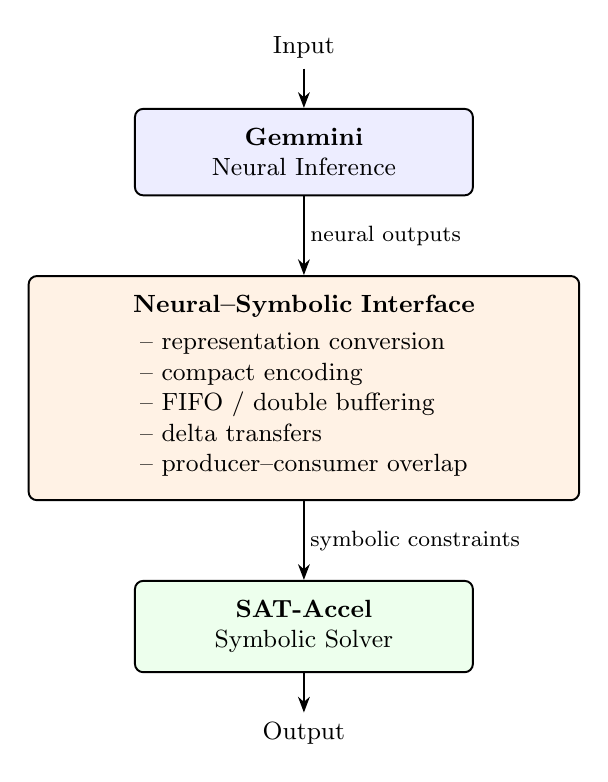
\begin{tikzpicture}[
  box/.style={draw, rounded corners=3pt, line width=0.7pt,
    align=center, font=\small, inner sep=7pt},
  flow/.style={-{Stealth[length=2mm]}, line width=0.7pt},
  label/.style={font=\footnotesize, fill=white, inner sep=2pt}
]
\node[font=\small] (input) {Input};
\node[box, fill=blue!7, below=5mm of input, text width=38mm] (gemmini)
  {\textbf{Gemmini}\\Neural Inference};
\node[box, fill=orange!10, below=10mm of gemmini, text width=65mm] (interface)
  {\textbf{Neural--Symbolic Interface}\\[3pt]
   \begin{tabular}{@{}l@{}}
   -- representation conversion\\
   -- compact encoding\\
   -- FIFO / double buffering\\
   -- delta transfers\\
   -- producer--consumer overlap
   \end{tabular}};
\node[box, fill=green!7, below=10mm of interface, text width=38mm] (sat)
  {\textbf{SAT-Accel}\\Symbolic Solver};
\node[font=\small, below=5mm of sat] (output) {Output};
\draw[flow] (input) -- (gemmini);
\draw[flow] (gemmini) -- node[label, right] {neural outputs} (interface);
\draw[flow] (interface) -- node[label, right] {symbolic constraints} (sat);
\draw[flow] (sat) -- (output);
\end{tikzpicture}

\caption{Neural--symbolic pipeline. Baselines implement the interface stage (orange) in CPU software through shared memory; ReasonLink implements it as a direct hardware stream.}
\label{fig:pipeline}
\end{figure}

\section{Evaluation Plan}
We will compare serial, double-buffered, and ReasonLink interfaces on visual Sudoku. All configurations use identical models, predictions, encodings, and solver settings, isolating the interface. Timing runs from inputs in DRAM to the solution in DRAM; cycle counters in each wrapper record busy, stall, and idle intervals.

To quantify the handoff, we decompose a serial run as
\begin{equation*}
T_{\text{e2e}} = T_{\text{nn}} + \underbrace{T_{\text{conv}} + T_{\text{xfer}} + T_{\text{sync}}}_{T_{\text{handoff}}} + T_{\text{sat}},
\end{equation*}
and we report the handoff fraction $T_{\text{handoff}}/T_{\text{e2e}}$. For overlapped runs, we report only the exposed handoff, $T_{\text{e2e}}-T_{\text{nn}}-T_{\text{sat}}$, to avoid double counting. We also report latency, throughput (puzzles/s), bytes moved per instance, synchronization and stall cycles, and per-accelerator utilization.

We will test three hypotheses. \emph{H1:} in the serial baseline, the handoff is a large fraction of Sudoku runtime, dominated by CPU conversion and full-image loading rather than by the size of the neural output. \emph{H2:} double buffering hides the handoff only while it is shorter than the slower stage, and moves no fewer bytes. \emph{H3:} ReasonLink's benefit shrinks as $T_{\text{sat}}$ grows; we will locate this crossover by varying instance hardness and size.

For ablations, we will add each mechanism individually and cumulatively, and sweep FIFO depth and transfer granularity. To separate algorithmic savings from hardware savings, we will also evaluate delta transfers as a CPU-only optimization. Puzzle accuracy, UNSAT rate (misclassified givens can make a puzzle unsatisfiable), and SAT assignments must be identical across interfaces and are checked against software references. Over-capacity instances and timeouts are reported separately.

\section{Timeline and Team Responsibilities}
\begin{center}
\begin{tabularx}{\columnwidth}{@{}P{0.15\columnwidth}Y@{}}
\toprule
\textbf{Date} & \textbf{Planned work and deliverables} \\
\midrule
Oct 19 & \emph{Infrastructure and baselines.} Gemmini runs the classifier; SAT-Accel RTL solves Sudoku CNFs in simulation; both baselines run end to end with cycle counters. \\
Nov 2 & \emph{Prototype and pilot results.} Baseline handoff breakdown (H1--H2); ReasonLink prototype with literal stream and on-chip FIFO; Nov~6 midterm talk. \\
Nov 23 & \emph{Initial results.} Delta transfers and overlap complete; three-way comparison across batch sizes and FIFO depths. \\
Dec 7 & \emph{Main results and ablations.} Per-mechanism ablations, crossover analysis (H3); poster for Dec~11. \\
Dec 18 & \emph{Final paper} and reproducible code, RTL, and scripts. \\
\bottomrule
\end{tabularx}
\end{center}

% \textbf{Risks and fallbacks.} The main risk is the SAT-Accel port: seven kernels, about ten AXI masters that originally targeted HBM, and fp64 activity arithmetic mapped to vendor floating-point IP. If RTL simulation is blocked, we will move to FireSim, where vendor IP synthesizes, or convert that arithmetic to fixed point.

\textbf{Team's Roles: } Both team members will contribute across Gemmini/Chipyard integration, SAT-Accel, the interface, and evaluation. Implementation and experimental tasks will be split for parallel work, while design decisions, debugging, experiments, and analysis remain shared. Regular review of each other’s work will ensure both of us maintain a complete understanding of the pipeline.

\clearpage
\bibliographystyle{IEEEtran}
\bibliography{neural-symbolic-references}
\end{document}